\documentclass{beamer}
\usepackage{up}

\title{Основни елементи на C++}

\date{11--18 октомври 2018 г.}

\begin{document}

\begin{frame}
  \titlepage
\end{frame}

\section{Синтаксис и семантика}

\begin{frame}
  \frametitle{Азбука}
  \begin{center}
    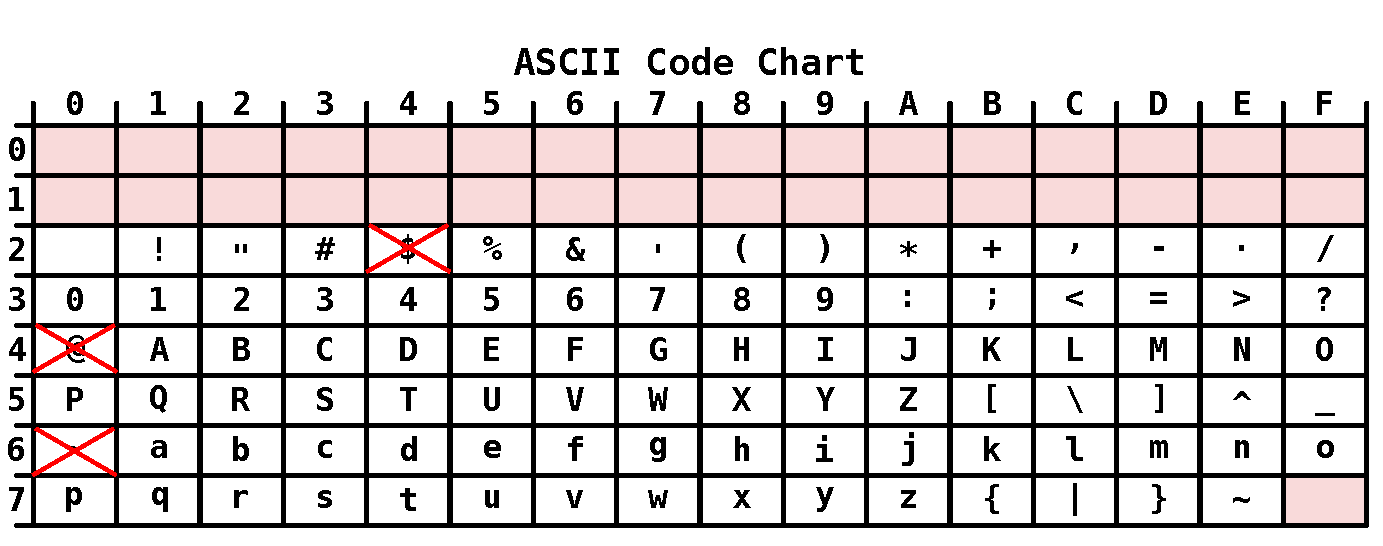
\includegraphics[width=0.9\textwidth]{images/ascii.pdf}\\[2em]
  \end{center}
  \wiki
\end{frame}

\begin{frame}
  \frametitle{Синтаксис}
  \begin{itemize}[<+->]
  \item Правила за построяване на текст
  \item \alert{Иван чете интересна книга.}
  \item \alert{Студентът пише програма.}
  \item \alert{книга. чете Иван? интерес на}
  \item\ <изречение> ::= <подлог> <сказуемо> [ <определение> ] <допълнение>\alert.
  \item\ <подлог> ::= <собствено\_съществително> | <нарицателно\_съществително><пълен\_член>
  \item\ <пълен\_член> ::= \alert{ът} | \alert{ят} | \alert{та} | \alert{то}
  \item\ <сказуемо> ::= <глагол>
  \item\ <определение> ::= <прилагателно>
  \item\ <допълнение> ::= <собствено\_съществително> | <нарицателно\_съществително>
  \end{itemize}
\end{frame}

\begin{frame}
  \frametitle{Синтактичен анализ — пример 1}
  \begin{itemize}[<+->]
  \item\ <изречение>
  \item\ <подлог> <сказуемо> [ <определение> ] <допълнение>\alert.
  \item\ <собствено\_съществително> <сказуемо> <определение> <допълнение>\alert.
  \item \alert{Иван} <глагол> <определение> <допълнение>\alert.
  \item \alert{Иван чете} <определение> <нарицателно\_съществително>\alert.
  \item \alert{Иван чете} <прилагателно> \alert{книга.}
  \item \alert{Иван чете интересна книга.}
  \end{itemize}
\end{frame}

\begin{frame}
  \frametitle{Синтактичен анализ — пример 2}
  \begin{itemize}[<+->]
  \item\ <изречение>
  \item\ <подлог> <сказуемо> [ <определение> ] <допълнение>\alert.
  \item\ <нарицателно\_съществително><пълен\_член> <сказуемо> <допълнение>\alert.
  \item \alert{Студент}{}<пълен\_член> <глагол> <допълнение>\alert.
  \item \alert{Студентът} <глагол> <нарицателно\_съществително>\alert.
  \item \alert{Студентът} <глагол> \alert{програма.}
  \item \alert{Студентът пише програма.}
  \end{itemize}
\end{frame}

\begin{frame}
  \frametitle{Синтактичен анализ — пример 3}
  \begin{itemize}[<+->]
  \item\ <изречение>
  \item\ <подлог> <сказуемо> [ <определение> ] <допълнение>\alert.
  \item\ <нарицателно\_съществително><пълен\_член> <сказуемо> <собствено\_съществително>\alert.
  \item \alert{Програма}{}<пълен\_член> <глагол> \alert{Иван.}
  \item \alert{Програмата гледа Иван.} \onslide<+-> 
\includegraphics[width=20ex, right]{images/creepy.png}
  \item Освен да е построено правилно, изречението трябва да има смисъл!
  \item \textbf{Семантика:} смисъл, значение на текст
  \end{itemize}
\end{frame}

\begin{frame}
  \frametitle{Мета-език на Backus-Naur}
  \begin{itemize}[<+->]
  \item\ <цифра> ::= \tta0 | \tta1 | \tta2 | \tta3 | \tta4 | \tta5 | \tta6 | \tta7 | \tta8 | \tta9
  \item\ <цяло\_число\_без\_знак> ::= <цифра> \{<цифра>\}
  \item\ <цяло\_число> ::= [\tta{+}|\tta{-}] <цяло\_число\_без\_знак>
    \begin{itemize}
    \item \tta{-15}, \tta{2}, \tta{+412}
    \end{itemize}
  \item\ <латинска\_буква> ::= \tta{A} | \tta{B} | ... | \tta{Y} | \tta{Z} | \tta{a} | \tta{b} | ... | \tta{y} | \tta{z}
  \item\ <идентификатор> ::=  \tta{\_} | <латинска\_буква> \{<латинска\_буква> | <цифра> | \tta{\_} \}
    \begin{itemize}
    \item \tta{a}, \tta{name}, \tta{X1}, \tta{\_Data15}
    \end{itemize}
  \end{itemize}
\end{frame}

\section{Синтактични елементи}

\begin{frame}
  \frametitle{Основни думи на C++ (tokens)}
  \begin{itemize}[<+->]
  \item\ <идентификатор> ::= \tta\_ | <латинска\_буква> \{<латинска\_буква> |
      <цифра> | \tta\_ \}
  \item запазени думи
  \item стандартни идентификатори
  \item литерали
    \begin{itemize}
    \item числови (\tt1, \tt{-5}, \tt{+2.34}, \tt{1e-02}, \tt{012}, \tt{0x123})
    \item символни (\tt{'a'}, \tt{'\textbackslash{}t'})
    \item низови (\tt{"hello"}, \tt{"yes!"})
    \end{itemize}
  \item операции (\tt+, \tt-, \tt*, \tt/)
  \item разделители (\tt{: ; , ( ) [ ] \{ \} < >})
  \end{itemize}
\end{frame}

\begin{frame}[fragile]
  \frametitle{Коментари}
  \begin{itemize}[<+->]
  \item\ <коментар> ::= \tta{//}<текст\_на\_един\_ред> |  \tta{/*} <текст> \tta{*/}
  \item Компилаторът игнорира:
    \begin{itemize}
    \item коментари
    \item празни символи (интервал, табулация, нов ред)
    \end{itemize}
  \item Пример:
\begin{lstlisting}
int sum = 0; // нулираме сумата
/*
   @\emph{вече сме готови да започнем пресмятането}@
   @\emph{последователно ще натрупваме поредните числа в sum}@
   @\emph{докато не ги изчерпим всичките}@
*/
...
\end{lstlisting}
  \end{itemize}
\end{frame}

\begin{frame}
  \frametitle{Променливи}
Променливата е именувана област в паметта.\\
\alert{\footnotesize Различно от променлива в математиката!}\\[1em]
\pause
\begin{itemize}
\item Име (идентификатор)
\item Място в паметта (адрес)
\item Тип
\item Стойност
\end{itemize}
\pause
\begin{center}
  \begin{tabular}{|p{2ex}|p{8ex}|p{8ex}|p{2ex}|p{4ex}|p{16ex}|}
    \multicolumn 1c{}&\multicolumn2l{\tt{fn}}&\multicolumn2l{\tt c}&\multicolumn1l{\tt{pi}}\\
    \hline
    \rowcolor{diagramblue}
    \ldots&\tt{81111}&\ldots&\tt{F}&\ldots&\tt{3.14159}\\
    \hline
    \multicolumn 1c{}&\multicolumn2l{\tt{int}}&\multicolumn2l{\tt{char}}&\multicolumn1l{\tt{double}}\\
  \end{tabular}
\end{center}
\end{frame}

\begin{frame}[fragile]
  \frametitle{Дефиниция и присвояване}
<дефиниция> ::= <тип>
<идентификатор> [ \tta= <израз> ] \{\tta,\\
\hspace{25ex}
<идентификатор> [ \tta= <израз> ] \}\tta;\\[2em]
<присвояване> ::= <идентификатор> \tta= <израз>\tta;\\[2em]
\pause
Примери:
\begin{itemize}
\item \lstinline{double x;}
\item \lstinline{int a, b = 15;}
\item \lstinline{a = b + 5;}
\item \lstinline{x = a * (b - 3);}
\item \sta{double y = double x;}
\end{itemize}
\end{frame}

\begin{frame}<1-5>[fragile]
  \frametitle{Изход на екрана}

  \begin{itemize}
  \item \tta{cout <{}<} <израз> \{\tta{<{}<} <израз>\}\tta;
    \begin{overlayarea}{\textwidth}{7em}
    \item \temporal<2>{\tt{cout <{}< a <{}< b <{}< c;}}{\tt{((cout <{}< a) <{}< b) <{}< c;}}{$\underbrace{\underbrace{\tt(\underbrace{\tt{(cout <{}< a)}}_{\tt{cout}} \tt{<{}< b)}}_{\tt{cout}}\tt{ <{}< c}}_{\tt{cout}}\tt;$}
    \end{overlayarea}
  \item<4-> \lstinline{cout << "a + b = "} \lstinline{<< a + b << endl;}
  \item<5-> \sta{cout <{}< \quot a = \quot{} 2;}
  \end{itemize}
\end{frame}

\begin{frame}
  \frametitle{Вход от клавиатурата}

  \begin{itemize}
  \item \tta{cin >{}>} <идентификатор> \{\tta{>{}>} <идентификатор>\}\tta;
    \begin{overlayarea}{\textwidth}{7em}
    \item \temporal<2>{\tt{cin >{}> a >{}> b >{}> c;}}{\tt{((cin >{}> a) >{}> b) >{}> c;}}{$\underbrace{\underbrace{\tt(\underbrace{\tt{(cin >{}> a)}}_{\tt{cin}} \tt{>{}> b)}}_{\tt{cin}}\tt{ >{}> c}}_{\tt{cin}}\tt;$}
    \end{overlayarea}
  \item<4-> \sta{cin >{}> a + b;}
  \item<5-> \sta{cin >{}> 15;}
  \end{itemize}
\end{frame}

\begin{frame}[fragile]
  \frametitle{Константи}
  \begin{itemize}[<+->]
  \item \tta{const} <тип> <идентификатор> \tta= <израз>\tta;
  \item стойността на константите:
    \begin{itemize}
    \item \alert{трябва} да бъде зададена при дефиниране
    \item \alert{не може} да се променя след това
    \end{itemize}
  \item Примери:
    \begin{itemize}
    \item \lstinline{const int FINGERS = 10;}
    \item \sta{FINGERS = FINGERS + 2;}
    \end{itemize}
  \end{itemize}
\end{frame}

\section{Типове}

\begin{frame}
  \frametitle{Типове}
  \begin{itemize}[<+->]
  \item Класификация на видовете данни
  \item Носят \textbf{семантична} информация
  \item Помагат за проверка на коректност
  \item Множество от допустими стойности
  \item Операции
  \item Вградени функции
  \end{itemize}
\end{frame}

\begin{frame}
  \frametitle{Класификация на типовете}
  \begin{itemize}
  \item Скаларни (атомарни)
    \begin{itemize}
    \item интегрални
      \begin{itemize}
      \item булев (\tt{bool})
      \item целочислен (\tt{int})
      \item символен (\tt{char})
      \item изброен (\tt{enum})
      \end{itemize}
    \item други
      \begin{itemize}
      \item числа с плаваща запетая (\tt{float}, \tt{double})
      \item указател (\tt{T*})
      \item псевдоним (\tt{T\&})
      \end{itemize}
    \end{itemize}
  \item Съставни
    \begin{itemize}
    \item масив (\tt{[]})
      \begin{itemize}
      \item низ (\tt{char[]})
      \end{itemize}
    \item структура (\tt{struct})
    \item клас (\tt{class})
    \item обединение (\tt{union})
    \end{itemize}
  \end{itemize}
\end{frame}

\begin{frame}
  \frametitle{Логически тип (\tt{bool})}
  \begin{itemize}
  \item Множество от стойности: \{\tt{false}, \tt{true}\}
  \item\ <булева\_константа> ::= \tta{true} | \tta{false}
  \item логически операции
  \end{itemize}
  \begin{center}
    \small
    \begin{tabular}{c@{\hskip 3ex}c@{\hskip 3ex}c}
      Конюнкция & Дизюнкция & Отрицание\\[1em]
      \begin{tabular}{c|c|c}
        \tt{\&\&}&\tt{false}&\tt{true}\\
        \hline
        \tt{false}&\tt{false}&\tt{false}\\
        \hline
        \tt{true}&\tt{false}&\tt{true}
      \end{tabular}
      &
        \begin{tabular}{c|c|c}
          \tt{||}&\tt{false}&\tt{true}\\
          \hline
          \tt{false}&\tt{false}&\tt{true}\\
          \hline
          \tt{true}&\tt{true}&\tt{true}
        \end{tabular}
      &
        \begin{tabular}{c|c}
          \tt{!}&\\
          \hline
          \tt{false}&\tt{true}\\
          \hline
          \tt{true}&\tt{false}
        \end{tabular}
    \end{tabular}
  \end{center}
\end{frame}

\begin{frame}
  \frametitle{Символен тип (\tt{char})}
  \begin{itemize}
  \item Множество от стойности
    \begin{itemize}
    \item \tt{signed char}: $[-128; 127]$
    \item \tt{unsigned char}: $[0; 255]$
    \end{itemize}
  \item Литерали
    \begin{itemize}
    \item \tta\apos<символ>\tta\apos
    \item \tta\apos\tta\textbackslash<контролен\_символ>\tta\apos
    \end{itemize}
\end{itemize}
\end{frame}

\begin{frame}
  \frametitle{Целочислен тип (\texttt{int})}
  \begin{itemize}
  \item Множество от стойности: $[-2^{31}; 2^{31}-1]$
  \item модификатори
    \begin{itemize}
    \item \tt{short}:\hspace{2ex} $[-2^{15}; 2^{15}-1 ]$
    \item \tt{long}:\hspace{2ex} $[-2^{63}; 2^{63} - 1]$
    \item \tt{unsigned}:\hspace{2ex} $[0; 2^x-1 ]$, където $(x = 16, 32, 64)$
    \end{itemize}
  \end{itemize}
\end{frame}

\begin{frame}
  \frametitle{Целочислен тип (\texttt{int})}
  \begin{itemize}
  \item аритметични операции
    \begin{itemize}
    \item едноместни операции за знак (\tt+, \tt-)
    \item двуместни аритметични операции
      \begin{itemize}
      \item \tt{a + b} (събиране)
      \item \tt{a - b} (изваждане)
      \item \tt{a * b} (умножение)
      \item \tt{a / b} (частно)
      \item \tt{a \% b} (остатък)
      \end{itemize}
    \end{itemize}
  \item операции за сравнение (предикати)
    \begin{itemize}
    \item \tt{a == b} (равно)
    \item \tt{a != b} (различно)
    \item \tt{a < b} (по-малко)
    \item \tt{a > b} (по-голямо)
    \item \tt{a <= b} (по-малко или равно)
    \item \tt{a >= b} (по-голямо или равно)
    \end{itemize}
  \end{itemize}
\end{frame}

\begin{frame}
  \frametitle{Числа с плаваща запетая}
  \begin{itemize}[<+->]
  \item \alert{Внимание: това не са реални числа!}
    \begin{itemize}
    \item А какво са реални числа?
    \end{itemize}
  \item Още ще ги наричаме и \textbf{дробни числа}
  \item Представяне в паметта
    \begin{itemize}
    \item $f = (-1)^s\cdot m\cdot 2^e$\\[1em]
      \begin{tabular}{|P{4ex}|P{12ex}|P{35ex}|}
        \hline
        \rowcolor{diagramblue}
        s&e&m\\
        \hline
        \multicolumn1c{$\underbrace{}_{\text{1 бит}}$}&\multicolumn1c{$\underbrace{\hspace{12ex}}_{\text{8 бита}}$}&\multicolumn1c{$\underbrace{\hspace{34.5ex}}_{\text{23 бита}}$}
      \end{tabular}\\[1em]
    \item $s \in \{0,1\}$ --- знак
    \item $m \in [0; 2^{23}-1]$ --- мантиса
    \item $e \in [-126; 127]$ --- експонента
    \item машинна нула: $(-2^{-127}; 2^{-127})$
    \end{itemize}
  \end{itemize}
\end{frame}

\begin{frame}
  \frametitle{Общо представяне на числа с плаваща запетая}
  $f = (-1)^s\cdot m\cdot 2^e$\\[1em]
  \begin{tabular}{|P{1.5ex}|P{12ex}|P{34.5ex}|}
    \hline
    \rowcolor{diagramblue}
    s&e&m\\
    \hline
    \multicolumn1c{}&\multicolumn1c{$\underbrace{\hspace{12ex}}_{\text{q бита}}$}&\multicolumn1c{$\underbrace{\hspace{34.5ex}}_{\text{p бита}}$}
  \end{tabular}
  \begin{itemize}
  \item $s \in \{0,1\}$ --- знак
  \item $m \in [0; 2^p-1]$ --- мантиса
    \begin{itemize}
    \item $p$ --- точност, брой двоични цифри на мантисата
    \end{itemize}
  \item $e \in [e_{min}; e_{max}]$ --- експонента
    \begin{itemize}
    \item $e_{min} = -e_{max}+1$
    \item $e_{max} = 2^{q-1}-1$
    \item $q$ --- обхват на експонентата
    \item $e_{min}-1$ и $e_{max}+1$ са запазени за служебно ползване
    \end{itemize}
  \item общо използвани битове: $p + q + 1$
  \item машинна нула: $(-2^{e_{min}-1}; 2^{e_{min}-1})$
  \end{itemize}
\end{frame}

\begin{frame}
  \frametitle{Типове дробни числа}
  \begin{tabular}{|P{1.5ex}|P{12ex}|P{34.5ex}|}
    \hline
    \rowcolor{diagramblue}
    s&e&m\\
    \hline
    \multicolumn1c{}&\multicolumn1c{$\underbrace{\hspace{12ex}}_{\text{q бита}}$}&\multicolumn1c{$\underbrace{\hspace{34.5ex}}_{\text{p бита}}$}
  \end{tabular}\\[2em]
  \begin{tabular}{|l|c|c|c|}
    \hline
    \textbf{тип}&\textbf{размер}&\textbf{точност (p)}&\textbf{обхват (q)}\\
    \hline\hline
    \tt{float}&4 байта = 32 бита&23 бита&8 бита\\
    \hline
    \tt{double}&8 байта = 64 бита&52 бита&11 бита\\
    \hline
    \tt{long double}&16 байта = 128 бита&112 бита &15 бита\\
    \hline
  \end{tabular}
\end{frame}

\begin{frame}
  \frametitle{Дробни литерали}
  \begin{itemize}
  \item\ [<цяло\_число>]\tta.[<цяло\_без\_знак>][(\tta{E}|\tta{e})<цяло\_число>]
  \item Примери: \tt1, \tt{2.34}, \tt{12e-2}, \tt{10.14E+03}, \tt{.23}
  \item Операции:
    \begin{itemize}
    \item всички за целочислен тип \alert{без \tt\%}
    \item \tt/ е \alert{дробно деление}, а не частно!
    \item сравненията \tt{==} и \tt{!=} са \alert{ненадеждни}!
    \end{itemize}
  \end{itemize}
\end{frame}


\begin{frame}[fragile]
  \frametitle{Математически функции}
  \lstinline{#include <cmath>}
  \begin{itemize}
  \item \tt{abs(x)}, \tt{fabs(x)}
  \item \tt{sin(x)}, \tt{cos(x)}, \tt{tan(x)}, \tt{asin(x)}, \tt{acos(x)}, \tt{atan(x)}
  \item \tt{exp(x)}, \tt{log(x)}, \tt{log10(x)}
  \item \tt{ceil(x)}, \tt{floor(x)}
  \item \tt{sqrt(x)}, \tt{pow(x, n)}
  \end{itemize}
\end{frame}

\section{Разрешаване на нееднозначности}

\begin{frame}
  \frametitle{Преобразуване на типове}
  \begin{itemize}
  \item $\tt{bool}\rightarrow%
    \tt{char}\rightarrow%
    \tt{short}\rightarrow%
    \tt{int}\rightarrow%
    \tt{long}\rightarrow%
    \tt{float}\rightarrow%
    \tt{double}$
  \item $\tt{unsigned char}\rightarrow%
    \tt{unsigned short}\rightarrow%
    \tt{unsigned}\rightarrow%
    \tt{unsigned long}$
  \item обратната посока може да доведе до \alert{загуба на информация}
  \item експлицитно преобразуване на типове:\\
    <преобразуване> ::= \tta(<тип>\tta)<израз>
%TODO: Примери
  \end{itemize}
\end{frame}

\begin{frame}
  \frametitle{Приоритет на операциите}
  \begin{enumerate}
  \item Обръщения към функции
  \item Скоби
  \item \tt!, \tt+, \tt- (едноместни)
  \item \tt*, \tt/, \tt\%
  \item \tt+, \tt- (двуместни)
  \item \tt{<{}<}, \tt{>{}>}
  \item \tt{<}, \tt{<=}, \tt{>}, \tt{>=}
  \item \tt{==}, \tt{!=}
  \item \tt{\&\&}
  \item \tt{||}
  \end{enumerate}
\end{frame}

\end{document}
